\chapter{Disertantes}

Presentamos aqu\'i los disertantes de cada evento con una breve biograf\'ia y
sus campos de investigaci\'on.

\section*{Encuentro de Estudiantes de \'Optica y Fotof\'isica (EEOF)}

%%%%%%%%%%%%%%%%%%% STEFANI
\subsection*{Fernando Stefani}


\begin{tabular}{ l l}
% \newcolumntype{S}{>{\centering\arraybackslash} m{.4\linewidth} }
{\multirow{3}{*}{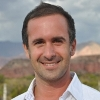
\includegraphics[width=0.08\textwidth]{fstefani}}} &  Applied
nanoPhysics Group. \\
 & Physics Department of the University of Buenos Aires. \\
 & fernando.stefani@df.uba.ar
\end{tabular}

\subsubsection*{Áreas de inter\'es}

Metallic, semiconducting and magnetic nanoparticles, Organic fluorophores,
Conjugated polymers, Supramolecular structures, Hybrid nanobiosystems, Proteins
and DNA.


\subsubsection*{Biograf\'ia}

Fernando Stefani was born in Buenos Aires on 19.11.1975. Materials
Engineer from the Instituto de Tecnolog\'ia Prof. Jorge Sabato (IT)-Buenos
Aires, Argentina. For his work at the Max-Planck-Institute for
Polymer Research (MPIP) under the supervision of Prof. Dr. W. Knoll,
he received his PhD on Natural Sciences in 2004 from the Johannes
Gutenberg Universitat Mainz. He stayed at the MPIP for a postdoctoral
stay until 2006, when he took a Research Fellow position at the
Institute of Photonic Sciences (ICFO) Barcelona, Spain, to work in the
group of Prof. Dr. Niek van Hulst. In 2008 he accepted a call from the
Ludwig-Maximilians-Universität München (LMU), Munich, Germany, and
joined the group of Prof. Dr. Jochen Feldmann as Assistan Professor of
the Physics Department. In 2009 Dr. Stefani returned to Argentina to
take a Researcher position at the National Research and Technical
Council (CONICET) and a Professorship at the Physics Department of the
University of Buenos Aires. Since 2011 Dr. Stefani directs a Partner
Group collaboration with the group of Prof. Dr. Stefan W. Hell of the
Max-Planck-Institute for Biophysical Chemistry. In 2005, Dr. Stefani
received the Otto Hahn Medal of the Max-Planck-Society.


%%%%%%%%%%%%%%%%%%%%%%%%% BRAGAS
\subsection*{Andrea Bragas}

\begin{tabular}{ l l}
% \newcolumntype{S}{>{\centering\arraybackslash} m{.4\linewidth} }
{\multirow{3}{*}{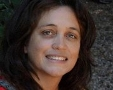
\includegraphics[width=0.08\textwidth]{abragas}}} & Quantum
Electronics Laboratory.  \\
 & Physics Department, FCEyN, UBA. Argentina. \\
 & bragas@df.uba.ar
\end{tabular}


\subsubsection*{Áreas de inter\'es}

High resolution optical microscopy, Plasmonic probes, Vibrations of plasmonic
objects and ensembles, Linear and nonlinear optical properties of nanomaterials.

\subsubsection*{Biograf\'ia}
    
Andrea Bragas is one of the heads of the Quantum Electronics Lab at the
University of Buenos Aires and professor at the School of Sciences. Her current
research fields are focused on the fabrication, study and control of different
isolated and interacting plasmonic objects with the aim of their application to
high-resolution microscopies, chemical and biological sensing, bio-imaging, and
development of nano-light sources. \\


%%%%%%%%%%%%%%%%%%%%%%%%%%%% MAIER
\subsection*{Stefan Maier}

\begin{tabular}{ l l}
% \newcolumntype{S}{>{\centering\arraybackslash} m{.4\linewidth} }
{\multirow{3}{*}{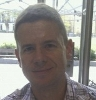
\includegraphics[width=0.08\textwidth]{smaier}}} &
Nanoplasmonics group.  \\
 & Imperial College, London, UK. \\
 & s.maier@imperial.ac.uk
\end{tabular}


\subsubsection*{Áreas de inter\'es}

Nanocavities: Fundamentals and applications in energy concentration and
biosensing, Optical and THz Metamaterials, Nanoantennas and enhanced
Light/Matter coupling, Active Plasmonics and Plasmon Waveguides,


\subsubsection*{Biograf\'ia}
    
Stefan Maier is Professor of Nanophotonics in the Department of Physics at
Imperial College London, and co-director of the College's Centre for Plasmonics
and Metamaterials. He obtained his PhD in Applied Physics at 2003 at the
California Institute of Technology. Stefan has published over 130 papers in
plasmonics and nanophotonics, is a fellow of OSA, and was awarded the Sackler
Prize in the Physical Sciences and the Paterson Medal of the Institute of
Physics. He further holds a Royal Society Wolfson Research Merit Award.\\


%%%%%%%%%%%%%%%%%%%%%%%%%% MENON
\subsection*{Rajesh Menon}

\begin{tabular}{ l l}
% \newcolumntype{S}{>{\centering\arraybackslash} m{.4\linewidth} }
{\multirow{3}{*}{
\includegraphics[width=0.08\textwidth]{rmenon}}} & Laboratory
for Optical Nanotechnologies.  \\
 & University of Utah, Utah, USA. \\
 & rmenon@eng.utah.edu
\end{tabular}

\subsubsection*{Áreas de inter\'es}

Absorbance Modulation Optical Lithography (AMOL), Patterning via Optical
Saturable Transformations (POST), Ultra-high efficiency photovoltaics via
Diffractive Spectrum Separation, Optimized Nanophotonics for efficient
ultra-thin-film photovoltaics, 3D tracking of surgical instruments.

\subsubsection*{Biograf\'ia}

Rajesh Menon has pioneered several technologies that will enable far-field
optics to manipulate and image matter with nanoscale resolution, something that
was thought impossible until a few years ago. His research has spawned over 50
publications, over 30 patents, and 2 spin-off companies. He has led several
projects in nanopatterning and nanoscopy with support from DARPA, the NSF, US
Air Force, and the MIT Deshpande Center for Technological Innovation. Among his
honors are an NSF CAREER Award (2011) and the International Commission for
Optics Prize (2009).\\
He currently directs the Laboratory for Optical Nanotechnologies at the
University of Utah. Prior to that, Prof. Menon was a research engineer at MIT's
Research Laboratory of Electronics, where he remains a research affiliate. He
holds S.M. and Ph.D. degrees from the Department of Electrical Engineering and
Computer Science at MIT. In addition, he served as the Chief Technology Officer
of LumArray, a company he co-founded with colleagues at MIT. \\



\section*{Taller de \'optica y Fotof\'isica (TOpFot)}

%%%%%%%%%%%%%%%%%%%%%%%%%%%% menon
\subsection*{Rajesh Menon}

\begin{tabular}{ l l}
% \newcolumntype{S}{>{\centering\arraybackslash} m{.4\linewidth} }
{\multirow{3}{*}{
\includegraphics[width=0.08\textwidth]{rmenon}}} & Laboratory
for Optical Nanotechnologies.  \\
 & University of Utah, Utah, USA. \\
 & rmenon@eng.utah.edu
\end{tabular}

(ver arriba)


%%%%%%%%%%%%%%%%%%%%%%%%%%%% MAIER
\subsection*{Stefan Maier}

\begin{tabular}{ l l}
% \newcolumntype{S}{>{\centering\arraybackslash} m{.4\linewidth} }
{\multirow{3}{*}{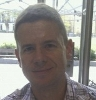
\includegraphics[width=0.08\textwidth]{smaier}}} &
Nanoplasmonics group.  \\
 & Imperial College, London, UK. \\
 & s.maier@imperial.ac.uk
\end{tabular}

(ver arriba)


%%%%%%%%%%%%%%%%%%%%%%%%%%%%%%% Galo
\subsection*{Galo Soler-Illia}

\begin{tabular}{ l l}
% \newcolumntype{S}{>{\centering\arraybackslash} m{.4\linewidth} }
{\multirow{3}{*}{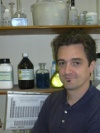
\includegraphics[width=0.08\textwidth]{galo}}} & Chemistry of
Nanomaterials Laboratory.  \\
 & CNEA. \\
 & gsoler@cnea.gov.ar 
\end{tabular}

\subsubsection*{Áreas de inter\'es}
Chemical Synthesis of Organized Matter, Mesoporous Thin Films, Surface
Modification, Plasmonics and Photonics, Metal-Oxide Interfaces, Catalysis.

\subsubsection*{Biograf\'ia}

Galo Soler-Illia leads the Chemistry of Nanomaterials Laboratory at the CNEA,
Buenos Aires, Argentina, and is Professor at the Dpt. of Inorganic Chemistry,
UBA since 2004. He has published more than a hundred papers in the field of
chemical synthesis of complex nanostructured matter. He has led national and
international scientific projects, including networking and collaboration with
the industry (PPG, TENARIS, RheinChemie, Darmex, Laring). He obtained several
national prizes, and has been a fellow of CONICET, CNRS, UBA and Fundaci\'on
Antorchas. His main current interest is the development of multiscale-patterned
functional materials with applications in environment, health and energy through
soft chemistry methods. More information can be found at
http://www.qi.fcen.uba.ar/personales/soler-illia.htm.

%%%%%%%%%%%%%%%%%%%%%%%%%%%%%%%% Rieznik
\subsection*{Andr\'es Rieznik}

\begin{tabular}{ l l}
% \newcolumntype{S}{>{\centering\arraybackslash} m{.4\linewidth} }
{\multirow{3}{*}{
\includegraphics[width=0.08\textwidth]{Rieznik}}} & Unidad de
Vinculaci\'on Estrat\'egica de ARSAT  \\
 & (Empresa Argentina de Soluciones Satelitales). \\
 & Investigador del CONICET. \\
 & aarieznik@arsat.com.ar
\end{tabular}

\subsubsection*{Biograf\'ia}
Andr\'es Rieznik naci\'o en Buenos Aires en 1976. Es Doctor en F\'isica por la
Universidad Estatal de Campinas (UNICAMP, Brasil), investigador del CONICET y
asesor de la Gerencia de Planeamiento Estrat\'egico de ARSAT en el \'area de las
comunicaciones \'opticas. Se especializa en el modelaje de la propagaci\'on no
lineal de la luz en fibras \'opticas y sus aplicaciones a sistemas y
dispositivos.


%%%%%%%%%%%%%%%%%%%%%%%%%%%%%%%% Saavedra
\subsection*{Carlos Saavedra} 

\begin{tabular}{ l l}
% \newcolumntype{S}{>{\centering\arraybackslash} m{.4\linewidth} }
{\multirow{3}{*}{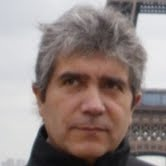
\includegraphics[width=0.08\textwidth]{carlos}}} & Departamento
de F\'isica, Facultad de Ciencias F\'isicas y Matem\'aticas, \\
 & Universidad de Concepci\'on, Chile.   \\
 & Centro de \'Optica y Fot\'onica, Universidad de Concepci\'on, Chile. \\
 & carlos.saavedra@cefop.udec.cl
\end{tabular}

\subsubsection*{Áreas de inter\'es}

Instrumentaci\'on \'Optica, \'Optica Cu\'antica,Informaci\'on Cu\'antica.

\subsubsection*{Biograf\'ia}

Profesor Titular en la Universidad de Concepci\'on desde el año 2001.
Inicialmente sus actividades de investigaci\'on se orientaron a la \'Optica
Cu\'antica. Posteriormente, desde el año 1997 a la fecha ha participado
activamente investigando en diversas tem\'aticas en Informaci\'on Cu\'antica,
desde el año 2005 con \'enfasis en el desarrollo de actividades experimentales .
Recientemente, sus actividades de investigaci\'on han estado orientadas
fuertemente en temas de instrumentaci\'on \'optica, donde junto a otros
investigadores de CEFOP
han dado un fuerte impulso a: Microscop\'ia de desenfoque, aplicaciones
biol\'ogicas; Pinzas \'Opticas y; DOAS. Adicionalmente, ha estado en forma
permanente ligado a actividades de difusi\'on especialmente orientadas a
estudiantes y p\'ublico general.


%%%%%%%%%%%%%%%%%%%%%%%%%%%%%% Galante
\subsection*{Mar\'ia Jos\'e Galante}

\begin{tabular}{ l l}
% \newcolumntype{S}{>{\centering\arraybackslash} m{.4\linewidth} }
{\multirow{3}{*}{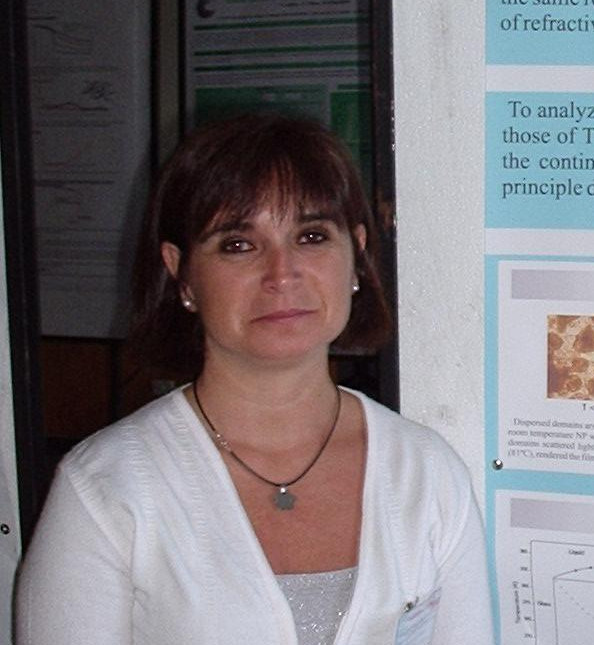
\includegraphics[width=0.08\textwidth]{galante}}} & Instituto
de Investigaciones en Ciencia y Tecnolog\'ia de Materiales, CONICET. \\
 & Universidad Nacional de Mar del Plata.   \\
 & galant@fi.mdp.edu.ar
\end{tabular}

\subsubsection*{Áreas de inter\'es}

Nanocompuestos polim\'ericos. Azopol\'imeros: pol\'imeros inteligentes que
contienen grupos azobenceno.

\subsubsection*{Biograf\'ia}

Investigadora Independiente (CONICET) (2006). Profesora Asociada (Departamento
de Ingenier\'ia en Materiales, Facultad de Ingenier\'ia, Universidad Nacional de
Mar del Plata) (2006). GRUPO DE INVESTIGACI\'ON: Pol\'imeros nanoestructurados
(INTEMA). ESTUDIOS/ESPECIALIZACI\'ON: Postdoctorado en Florida State University
(USA) (1994-1995). Doctora en Ciencia de Materiales, INTEMA,  Facultad de
Ingenier\'ia, Universidad Nacional de Mar del Plata (1989-1993). Licenciada en
Qu\'imica, Facultad de Ciencias Exactas y Naturales, Universidad Nacional de Mar
del Plata (1983-1989). ESTADÍAS EN EL EXTRANJERO: INSA de Lyon (Francia) (1998).
Universidad del Pa\'is Vasco, San Sebasti\'an (España) (2008).

%%%%%%%%%%%%%%%%%%%%%%%%%%%%% Requejo
\subsection*{Felix Requejo}

\begin{tabular}{ l l}
% \newcolumntype{S}{>{\centering\arraybackslash} m{.4\linewidth} }
{\multirow{3}{*}{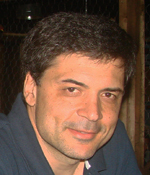
\includegraphics[width=0.08\textwidth]{requejo}}} & Instituto
de Investigaciones Fisicoqu\'imicas Te\'oricas y Aplicadas, CONICET. \\
 & Facultad de Ciencias Exactas, Departamento de Qu\'imica,   \\
 & Universidad Nacional de la Plata. \\
 & requejo@fisica.unlp.edu.ar
\end{tabular}

\subsubsection*{Biograf\'ia}

Es Investigador Principal CONICET y Profesor Adjunto Ordinario del Dto de Fisica
(FCE, UNLP). Actualmente se desempeña como Director Interino del INIFTA. Posee
m\'as de 80 publicaciones en revistas internacionales con referato y 300
presentaciones comunicaciones en congresos nacionales e internacionales. Es
Director del Grupo SUNSET del INIFTA y del Laboratorio de Absorci\'on de RX.

Asesor cient\'ifico del Programa de Nanotecnolog\'ia para el ``Fortalecimiento
de la Competitividad de las PYMES y Creaci\'on de Empleo en Argentina''
(MinCyT), miembro del Sistema Nacional de Rayos X (MinCyT). Miembro del Comit\'e
Binacional Argentino-Brasilero para la cooperaci\'on en el Proyecto del
Sincrotr\'on brasilero SIRIUS.
Premio ``Cristina Giordano'' 2011-2012 de la Asociaci\'on Fisicoqu\'imica
Argentina.
Premio Konex 2013 en Nanotecnolog\'ia.


%%%%%%%%%%%%%%%%%%%%%%%%%%%% levenson
\subsection*{Ariel Levenson}

\begin{tabular}{ l l}
% \newcolumntype{S}{>{\centering\arraybackslash} m{.4\linewidth} }
{\multirow{3}{*}{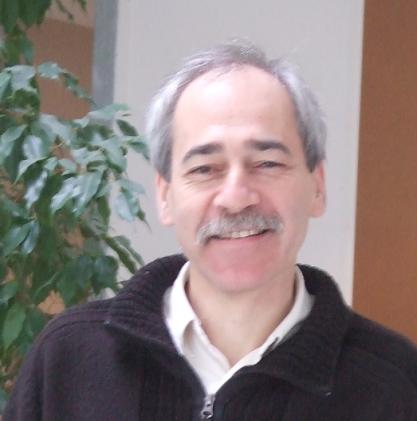
\includegraphics[width=0.08\textwidth]{levenson}}} &
Laboratoire de Photonique et de Nanostructures, \\
 & Centre National de la Recherche Scientifique- UPR20. France.\\
 & ariel.levenson@lpn.cnrs.fr 
\end{tabular}

\subsubsection*{Áreas de inter\'es}
Slow light propagation, Excitability, Rogue waves, Triple-photon quantum states,
Electromagnetically Induced Transparency and Coherent Population Oscillations,
Semiconductor photonic crystals, Microstructured fibres, Waveguide arrays,
Er-doped crystals.

\subsubsection*{Biograf\'ia}

Born in Argentina in 1957, he joined in 1988 the CNET laboratory, former R\&D
centre of France Telecom, where he has been working in ultrafast optical
nonlinearities in semiconductors and in quantum optics. In 1997 he become CNRS
senior scientist at the ``Laboratoire de Photonique et de Nanostructures'',
where he is the leader of the PHOTONIQ group. His present main domain of
researches is classical, nonlinear and quantum optics, in nano and
microstructures. 

He is the past director of the ``Centre of Nanoscience -\"\i le-de-France
Region;  C'Nano-IdF'' and is the director of the C'Nano national network that
coordinates the activities of the 6 regional C'Nanos and all the research teams
that belong to French academic laboratories developing activities in the
nanoscience and nanotechnology domain.